%!TEX root = ../../14-icra-RealTimeNMPC.tex

\newcommand{\tetazero}{20.55}
\newcommand{\Fkxzero}{-20}
\newcommand{\Fkyzero}{20}

\newcommand{\tetaone}{-20}
\newcommand{\Fkxone}{5}
\newcommand{\Fkyone}{0}

\newcommand{\tetatwo}{20}
\newcommand{\Fkxtwo}{25}
\newcommand{\Fkytwo}{20}

%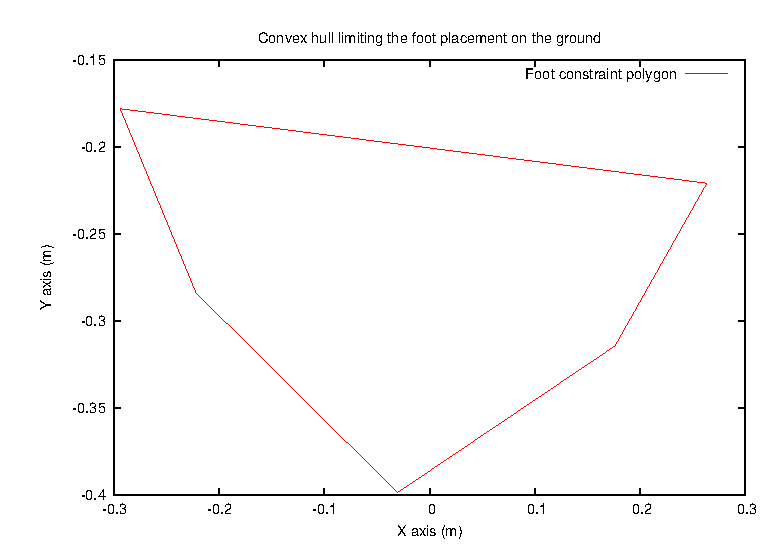
\includegraphics[width=15cm]{./figures/walking-without-thinking/ConvexHull}
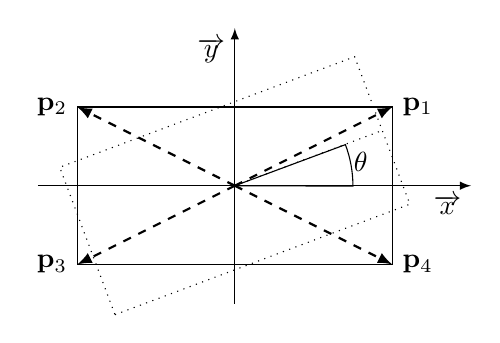
\begin{tikzpicture}[scale=0.050, node distance=2cm,>=latex]
\draw [->](-50,0) -- (60,0) node [below left, black]{$\overrightarrow{x}$}; %x-axis
\draw [->](0,-30) -- (0,40) node [below left, black]{$\overrightarrow{y}$}; %y-axis
 %support foot
\draw (-40,-20)--(40,-20)--(40,20)--(-40,20)--(-40,-20);

\draw [thick][dashed][->](0,0) -- (40,20) node [right, black]{${\bf p}_1$}; %y-axis
\draw [thick][dashed][->](0,0) -- (-40,20) node [left, black]{${\bf p}_2$}; %y-axis
\draw [thick][dashed][->](0,0) -- (-40,-20) node [left, black]{${\bf p}_3$}; %y-axis
\draw [thick][dashed][->](0,0) -- (40,-20) node [right, black]{${\bf p}_4$}; %y-axis

% rotated support foot
\draw [dotted][cm={cos(\tetazero) ,sin(\tetazero) ,-sin(\tetazero) ,cos(\tetazero) ,(0.0 cm,0.0 cm)}]
(-40,-20)--(40,-20)--(40,20)--(-40,20)--(-40,-20) ;
% rotated axis
\draw [dotted][-][cm={cos(\tetazero) ,sin(\tetazero) ,-sin(\tetazero) ,cos(\tetazero) ,(0.0 cm,0.0 cm)}]
(0,0) -- (40,0) node [below left, black]{};
% angle
\draw (0,0) -- (28.090986571,10.432619456) arc (\tetazero:0:30) -- (0.0,0.0) node at (32,6) {$\theta$} ;

\end{tikzpicture}
